\chapter{GraphFlow}
\label{chapter:graphflow}

In the previous chapter we've defined the concept of balance coefficient that motivate us to introduce the BalanceFlow model. In fact, the balance coefficient is also present in the FlipFlow energy and it seems that its computation is in the core of the evolution processes described so far. We confirm this hypothesis once more in this chapter. We present a graph-based model that converges to the digital shape of global optimum in the free digital Elastica problem. Moreover, the model is easily adapted for image segmentation tasks.

\section{Definitions}

Let $S$ a digital shape. Similarly to previous chapters, we denote $S^{(k)}$ the $k$-th shape produced by the model. If $k$ is ommited, we assume $k=0$. Given $n>0$, the optimization set $O_n^{(k)}$ is defined as

\begin{align*}
	O_n^{(k)} &:=\left\{ p \in \Omega \; | \; -n <= d_{S^{(k)}}(p) \leq n \right\}\\
\end{align*}

We are going to construct a graph $G_n( V,\mathcal{E})$ from $S$. The vertex set is defined as

\begin{align*}
	V&= \{ v_p \; | \; p \in S \} \cup T,
\end{align*}

where $T=\{s,t\}$ is the set of terminal vertices (source and target vertices, respectively).  We define an edge as a pair of vertices and a weight value, i.e., the triple $(v_1,v_2,w)$ denotes an edge from vertex $v_1$ to $v_2$ with weight $w$. The edge set of $G_n$ is defined as

\begin{align*}
	\mathcal{E}_1 &= \{ (v_p,v_q,w(p,q)) \; | \; \forall p \in O(S) \quad q \in \mathcal{N}_{4}(p) \}\\
	\mathcal{E}_2 &= \{ (s,v_p,M) \; | \; \forall p \in S \setminus O_n(S) \} \\
	\mathcal{E}_3 &= \{ (v_p,t,M) \; | \; \forall p \in \overline{S} \setminus O_n(S) \} \\
	\mathcal{E} &= \mathcal{E}_1 \cup \mathcal{E}_2 \cup \mathcal{E}_3,
\end{align*}

where $w(p,q) = u(S,p) + u(S,q)$ and $M=\pi^2 R^4$. 

\begin{definition}{Cut set}
 A cut set of a graph $G(V,\mathcal{E})$ is a subset $\mathcal{E}' \subset \mathcal{E}$ such that source and target vertices are not connected in $G(V,\mathcal{E} \setminus \mathcal{E}')$. The value of a cut is defined as
 
 \begin{align*}
 	v(\mathcal{E}') &= \sum_{e \in \mathcal{E}'}{w(e)}.
 \end{align*}
 
\end{definition}

Cuts are a natural way to partition a digital shape in two disjoint sets. In the GrabCut algorithm, the images are partitioned in foreground and background. In the context of shape evolution, we partition the vertices in: those belong to $S$ (connected to source) and those who do not belong to $S$ (connected to target).

The graph $G_n$ is built such that its minimum cut comprises the pixels of minimum balance coefficients sum. We denote $C_s^{(k)}(G_n)$ ($C_t^{(k)}(G_n)$) the source (target) component of the graph induced by the minimum cut of $G_n$. 

\begin{definition}{$n$-GraphFlow}

Given a natural number $n>0$ and digital set $S$, the $n$-GraphFlow is defined as

\begin{align*}
	\left \{ S^{(k)} \; | \; \begin{array}{ll}
	S^{(0)}&=S \\
	S^{(k)}&= \{ p \; | \; v_p \in C_s^{(k)}(G_n) \}
	\end{array} \right\}
\end{align*}

\end{definition}

The $n$-GraphFlow produces similar results to the previous flows (see figure \ref{fig:graph-flow-neigh0-results}), but is much faster to compute and implement. In the next section, we present a local-search strategy for the GraphFlow model that evolves the initial shape to its global optimum in the free Elastica problem.

\begin{figure}
\begin{tabular}{cccc}
&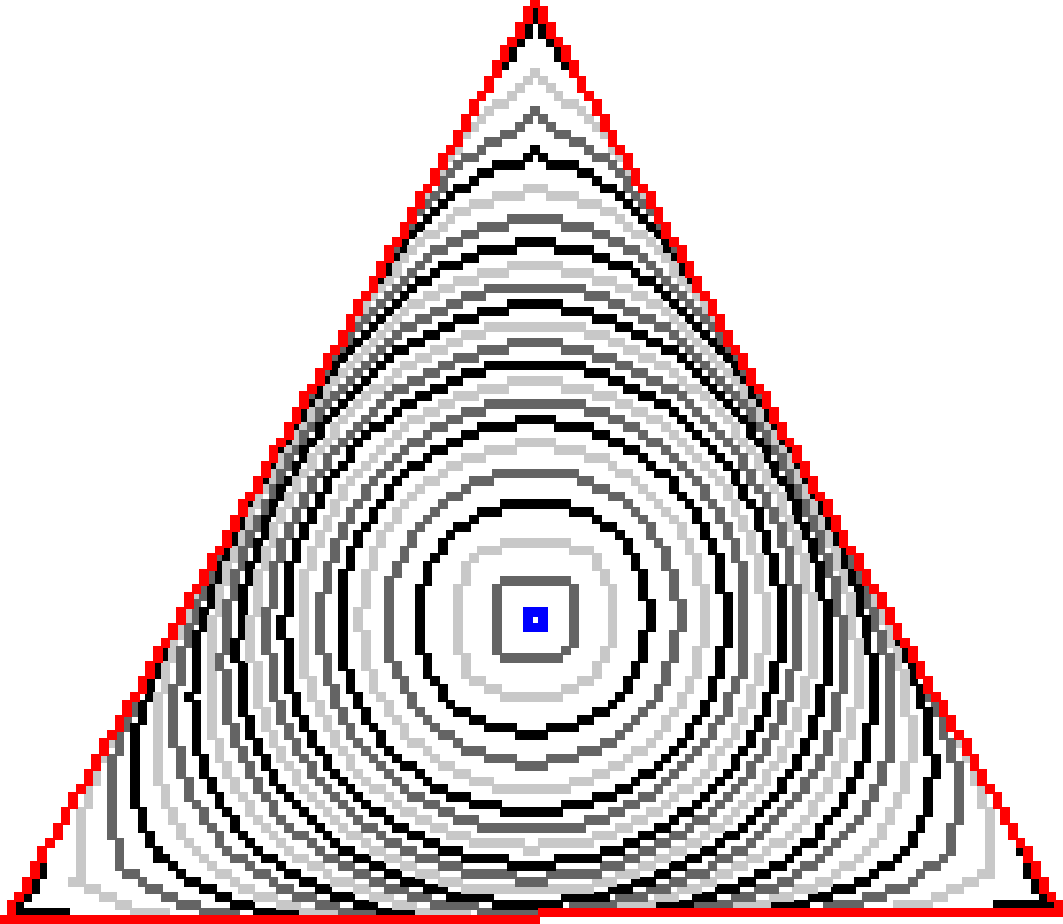
\includegraphics[scale=0.25]{figures/chapter8/graph-flow/triangle/neigh-0/summary.pdf} & 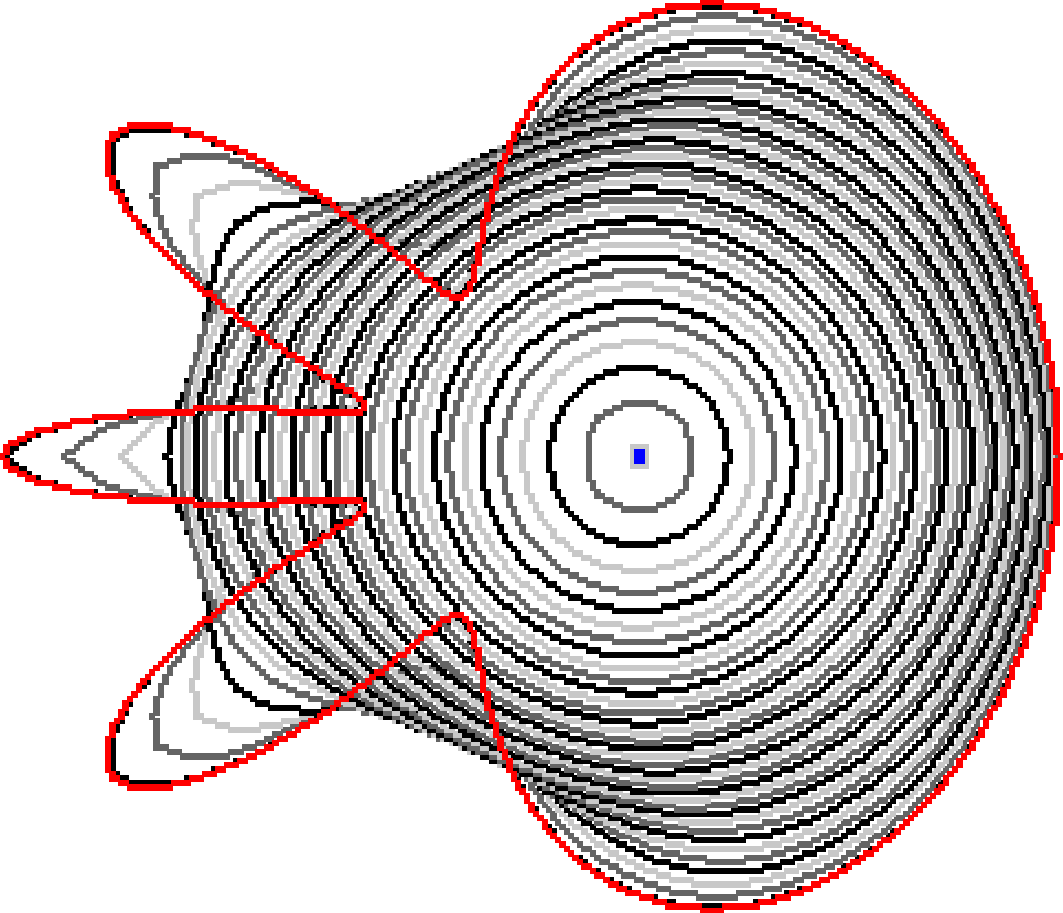
\includegraphics[scale=0.25]{figures/chapter8/graph-flow/flower/neigh-0/summary.pdf} & 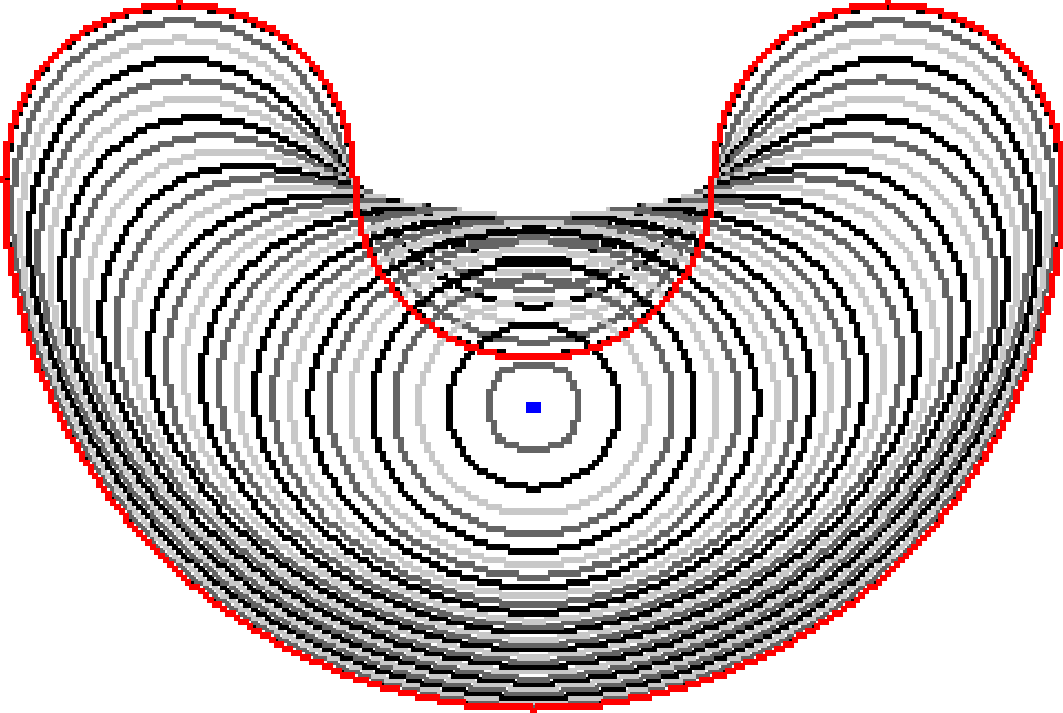
\includegraphics[scale=0.25]{figures/chapter8/graph-flow/bean/neigh-0/summary.pdf}
\end{tabular}
\caption{$1$-GraphFlow results for the triangle, flower and bean shapes. Differently from the previous models, the GraphFlow evolves the shape to a single point for any value of $m$. However, for higher values of $m$ the convergence is faster. Shapes are displayed at every $10$ iterations.}
\label{fig:graph-flow-neigh0-results}
\end{figure}

\section{LSGC algorithm}
	We present a local-search strategy for the GraphFlow model. The idea is to define a neighborhood for shape $S^{(k)}$ and compute the GraphFlow model for each of its members. The next shape $S^{(k+1)}$ is chosen as the one with lower digital Elastica.

\begin{definition}{$a$-neighborhood explorer set}
	Let $S$ a digital set and $a$ a natural number. Its $a$-neighborhood explorer set is defined as
	\begin{align*}
		N_a(S) &= S \cup \bigcup_{a' < a}{S^{+a} \cup S^{-a}},
	\end{align*}
	where $S^{+a}$($S^{-a}$) denotes a dilation(erosion) by a square of side $a$.
\end{definition}

The local-search graph-flow (LSGF) algorithm is described as


\begin{algorithm}
 \SetKwData{It}{k}
 \SetKwData{MIt}{maxIt}
 \SetKwData{Delta}{delta}
 \SetKwInOut{Input}{input}\SetKwInOut{Output}{output}
 \SetKwComment{comment}{//}{}
 
 \Input{A digital set $S$; the optimization band $m$; the neighborhood explorer set size $a$; parameter vector $\Theta=(\alpha,\beta)$; the maximum number of iterations \MIt;} 
 \BlankLine
 $S^{(0)} \longleftarrow S$\;
 $k \longleftarrow 1$\;
 \While{ \It $<$ \MIt  }{ 	
	$candidates \longleftarrow \{\}$\;
	\comment{Candidate selection}
 	\ForEach{ $X \in N_a(S^{(k)})$ }
 	{
 		$candidates \longleftarrow candidates \cup \{ p \; | \; v_p \in C_s( X ) \}$\;
 	}

	\comment{Candidate validation}
	$S^{(k)} \longleftarrow \displaystyle \argmin_{X \in candidates}{ \hat{E}_{\Theta}(X) }$\; 	
	\It $\longleftarrow$ \It $+1$\;
	
 }
 \caption{LSGF algorithm.}
 \label{alg:legc-algorithm}  
\end{algorithm}

We remark that the LSGF algorithm possess two fundamental steps: the candidate selection and the candidate validation. The former can be interpreted as an advanced filter that choses the best candidates for digital Elastica minimization in the explored neighborhood. Among those choices, we chose the one with lower digital Elastica energy in the candidate validation step.

The LSGF algorithm can grow or shrink accordingly with the $\alpha$ coefficient in the digital Elastica (see figure \ref{fig:graph-flow-neigh2-results}). For $a=0$, we recover the convergence to a point behaviour observed in both FlipFlow and BalanceFlow model. Moreover, its solution for the free Elastica problem is very similar to those given by the enumerative process of chapter \ref{chapter:digital-elastica}, i.e., the shapes converges to the expected global optimum. However, for the constrained Elastica problem, the LSGF encounters some difficulties to evolve (see figure \ref{fig:graph-flow-constrained}). We believe that a larger neighborhood, possibly random, could solve this issue.

\begin{figure}
\begin{tabular}{cccc}
&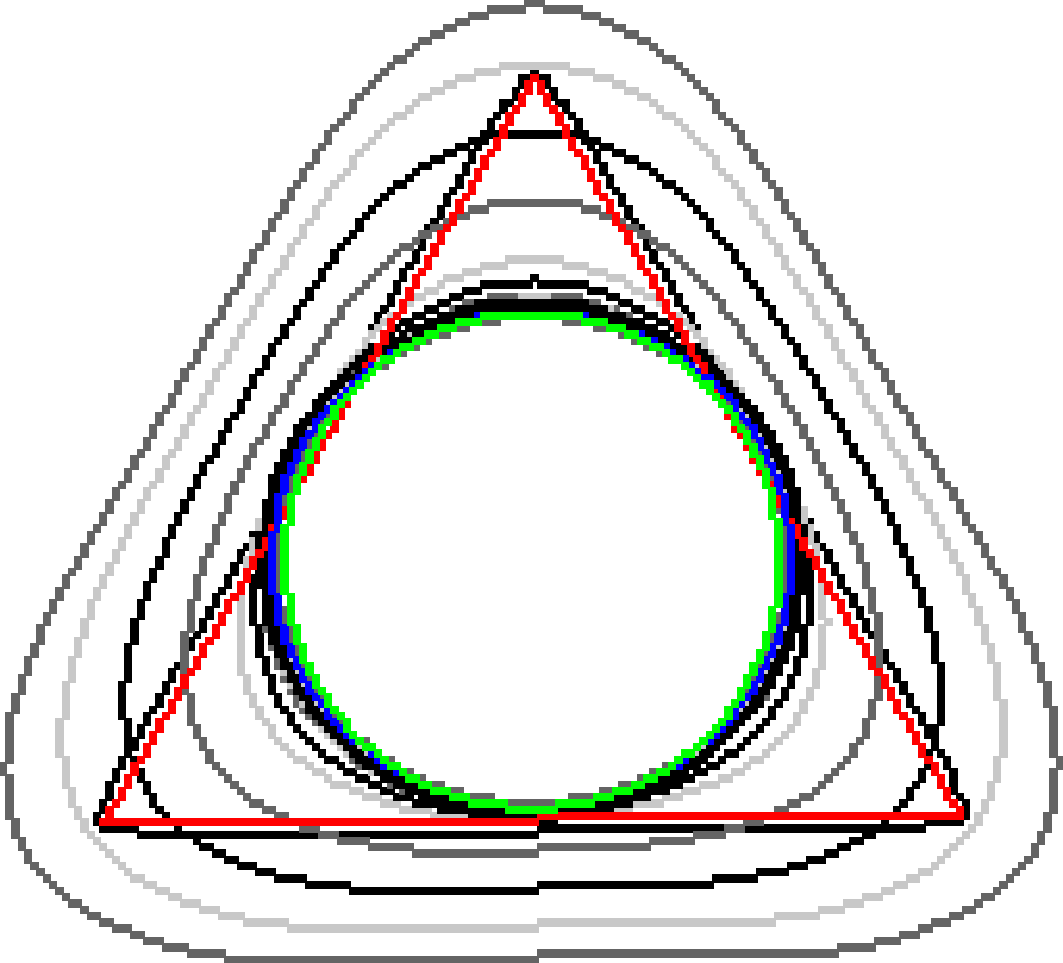
\includegraphics[scale=0.25]{figures/chapter8/graph-flow/triangle/neigh-2/summary.pdf} & 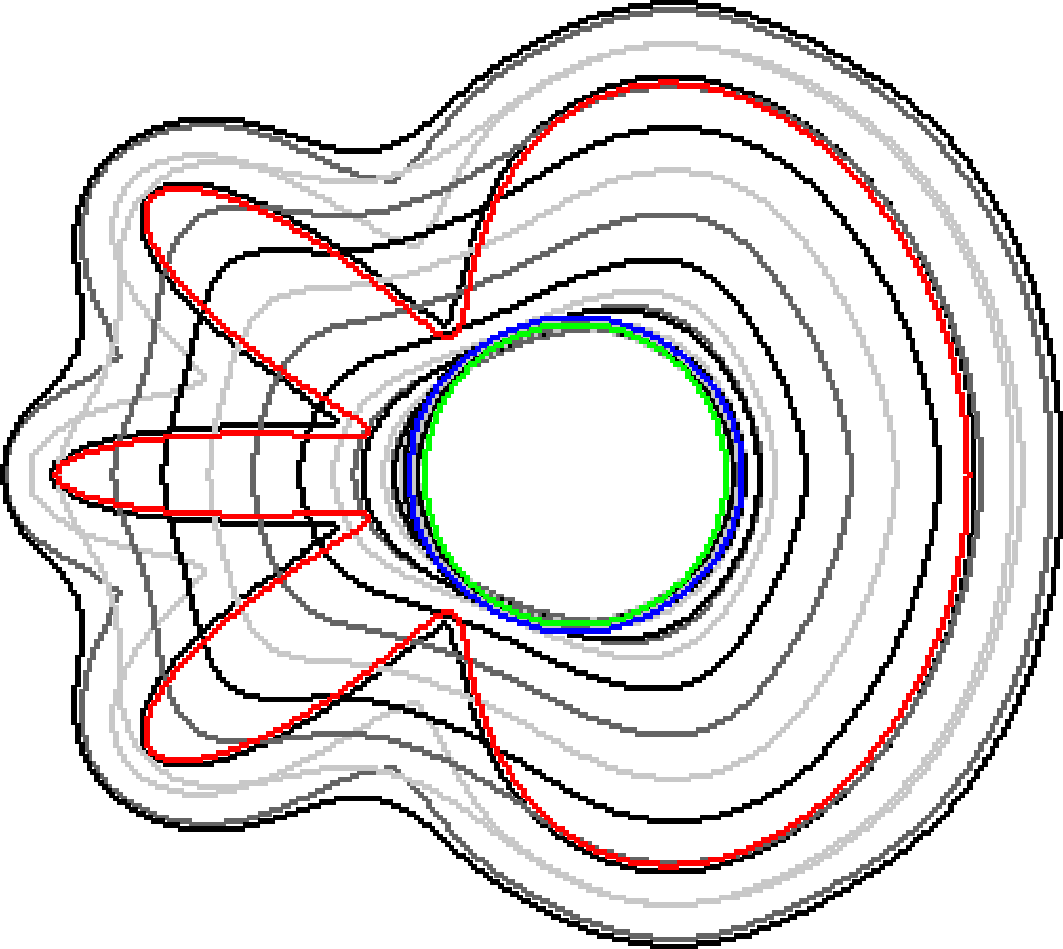
\includegraphics[scale=0.25]{figures/chapter8/graph-flow/flower/neigh-2/summary.pdf} & 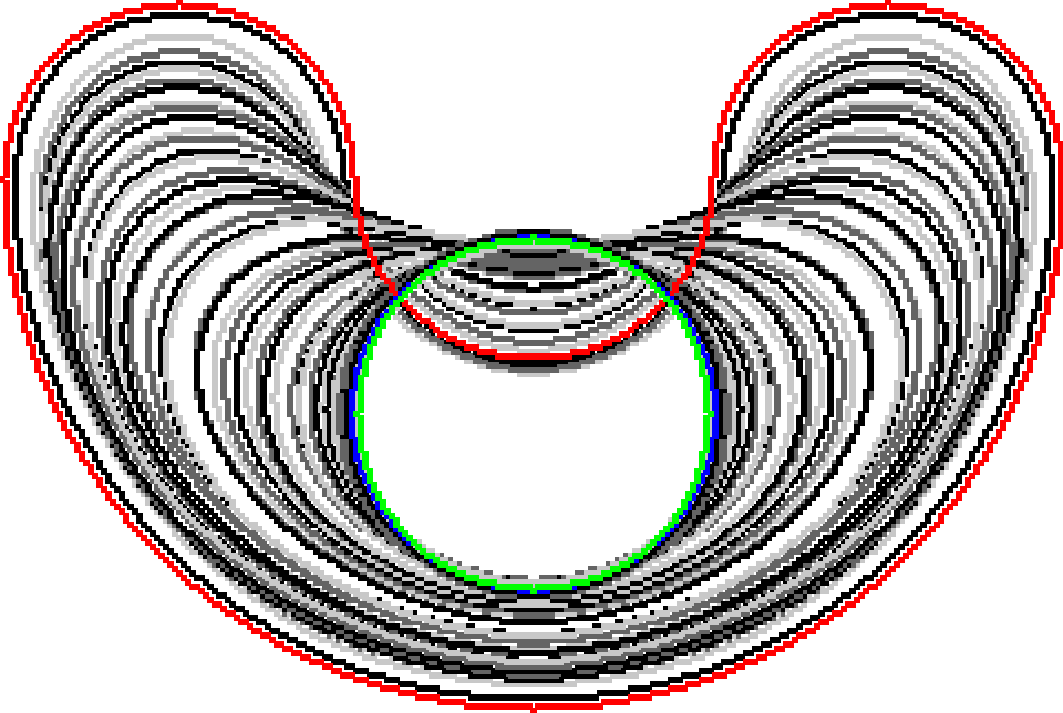
\includegraphics[scale=0.25]{figures/chapter8/graph-flow/bean/neigh-2/summary.pdf}
\end{tabular}
\caption{The LSGF algorithm can shrink and grow, and it converges to the global optimum (green curve) in the free Elastica problem. For the flows in the figure, we are using $a=2$ and shapes are displayed at every $10$ iterations.}
\label{fig:graph-flow-neigh2-results}
\end{figure}


\begin{figure}
\begin{tabular}{ccc}
&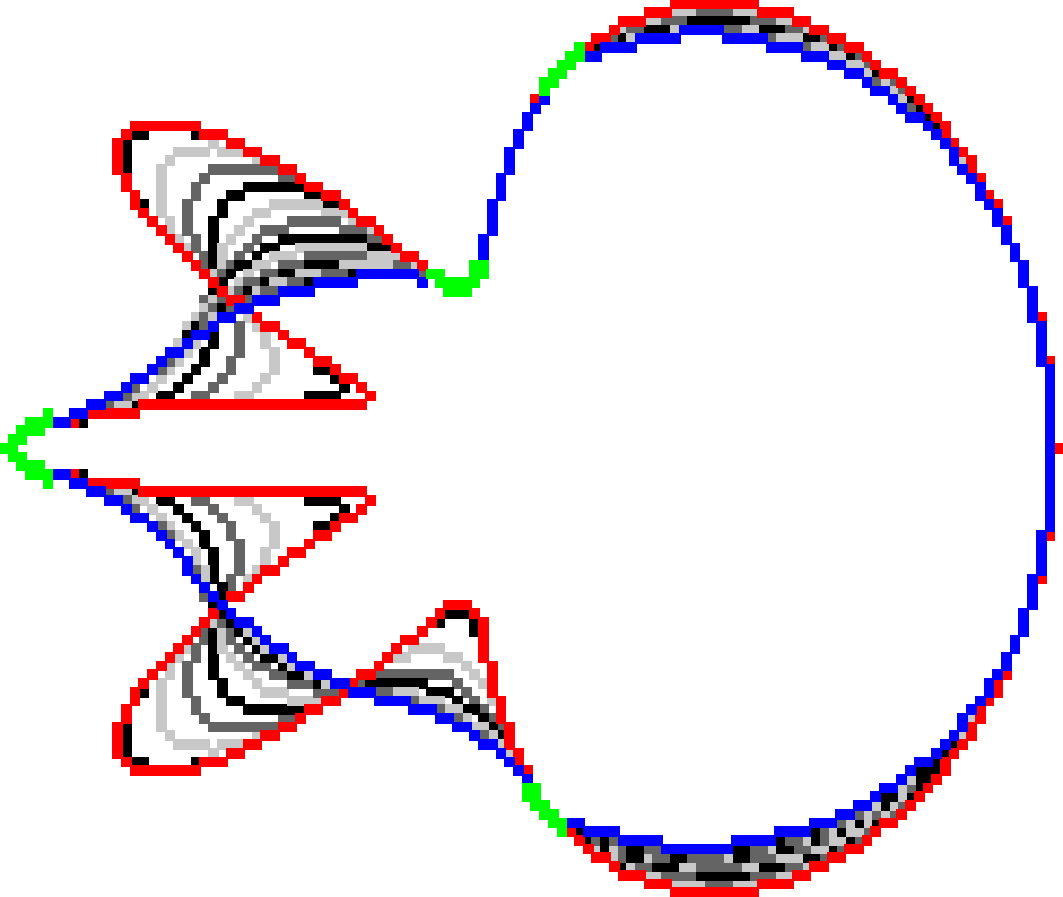
\includegraphics[scale=0.4]{figures/chapter8/constrained-elastica/flower-1/lp-0.001/summary.pdf} & 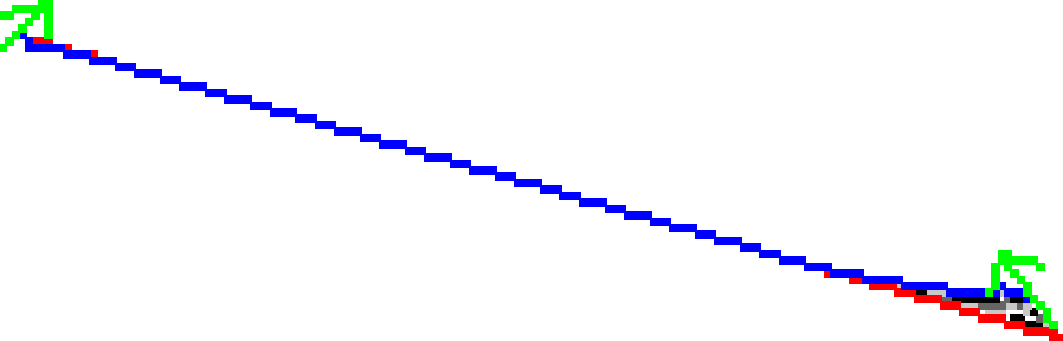
\includegraphics[scale=0.4]{figures/chapter8/constrained-elastica/curve-3/lp-0.001/summary.pdf}
\end{tabular}
\caption{The LSGF encounters some difficulties to evolve the shapes in the constrained Elastica problem. We think that a larger, possibly random, neighborhood may solve the problem. For both flows in the figure, we are using $a=2$.}
\label{fig:graph-flow-constrained}
\end{figure}

\section{Injecting data term}

The GrabCut model (see \ref{chapter:appendix-grabcut-model}) is the state-of-art graph-based technique for image segmentation tasks . The GrabCut model possesses two data term components, one related to the boundary, and another to the region. Several works tried to inject geometric information in a graph-cut framework for image segmentation. While some works were sucessfuly in injecting perimeter penalization, those that attempt to include curvature suffered from lack of precision, lack of theoretical guarantees and high running times. In this section we propose a model that advances in these two criterias.

Let $I:\Omega \rightarrow [0,1]^3$ a color image. We define $I(O_m)$ as the subset of $I$ restricted to the optimization region $O_m$. Let $X_m = X(I(O_m))$ and $x$ a possible binary assignment. We recall the GrabCut minimization energy for given parameters $\Lambda=(\lambda_r, \lambda_b)$, image $I$ and labeling $x$.

\begin{align*}
	grabc_{\Lambda}(I,x) &= \lambda_r \sum_{p \in \Omega}{regional(I,x,p)} + \lambda_b \sum_{p,q \in \Omega}{boundary(I,x,p,q)}.
\end{align*}

To construct the graph $G(V,\mathcal{E})$, we define the edge's weight function $w$ such that curvature and data terms are contemplated. Therefore,  

\[
	\forall p,q \in O_m, \quad w(v_p,v_q) = \left\{ \begin{array}{ll}
		\beta(u(S,p) + u(S,q)) + \lambda_b boundary(I,x,p,q), & \text{if } p,q \notin T	\\
		\beta M + \lambda_r regional(I,x,p,q), & \text{if } p \in T \text{ xor } q \in T \\
		0, & \text{otherwise}
	\end{array},\right.
\]

The validation function is defined as

\begin{align*}
val_{(\Theta,\Lambda)}(S^{(k-1)},I,x^{(k-1)}) &= \hat{E}_{\Theta}(S) + grabc_{\Lambda}(I,x)
\end{align*}

Finally, the squared curvature correction algorithm is described as

\begin{algorithm}
 \SetKwData{It}{k}
 \SetKwData{MIt}{maxIt}
 \SetKwData{Delta}{delta}
 \SetKwData{Tol}{tolerance}
 \SetKwInOut{Input}{input}\SetKwInOut{Output}{output}
 \SetKwComment{comment}{//}{}
 
 \Input{A digital set $S$; the optimization band $m$; the neighborhood explorer set size $a$;  parameter vector $\Theta=(\alpha,\beta)$; data term coefficients $\Lambda=(\lambda_r,\lambda_b)$; tolerance $tolerance$.}
 \BlankLine
 $S^{(0)} \longleftarrow S$\;
 $k \longleftarrow 1$\;
 \Delta $\longleftarrow +\infty$\;
 \While{ \It $<$ \MIt \bf{and} \Delta $>$ \Tol  }{ 	
	$candidates \longleftarrow \{\}$\;
	\comment{Candidate selection}
 	\ForEach{ $X \in N_a(S^{(k)})$ }
 	{
 		$candidates \longleftarrow candidates \cup x\big( \; \{ p \; | \; v_p \in C_s( X ) \} \; \big)$\;
 	}

	\comment{Candidate validation}
	$S^{(k)} \longleftarrow \displaystyle \argmin_{x \in candidates}{ val_{(\Theta,\Lambda)}(S^{(k-1)},I,x^{(k-1)})}$\; 	
	\It $\longleftarrow$ \It $+1$\;
	\Delta $\longleftarrow | val_{(\Theta,\Lambda)}(S^{(k)},I,x^{(k)}) - val_{(\Theta,\Lambda)}(S^{(k-1)},I,x^{(k-1)}) |$\;
	
 }
 \caption{LSGF squared curvature segmentation correction algorithm.}
 \label{alg:legc-segmentation-algorithm}  
\end{algorithm}


\begin{figure}[]
\center
\begin{tabular}{cccc}
\multirow{2}{*}{Seeds} & \multirow{2}{*}{GrabCut} & $\alpha=0.5, \beta=0.0,$ & $\alpha=0.5, \beta=1.0,$\\
& & $\lambda_r=\lambda_b=2.0$ & $\lambda_r=\lambda_b=2.0$\\
 	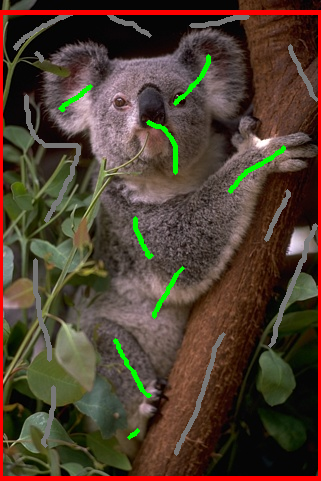
\includegraphics[scale=0.25]{figures/chapter8/segmentation/coala/k-0.0/seeds.png} & 
 	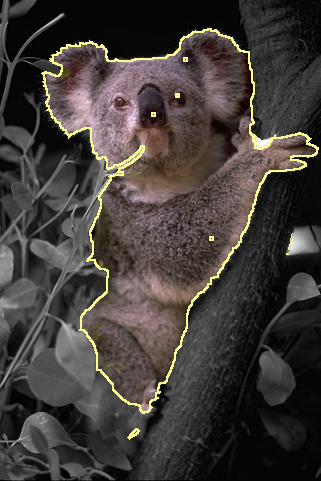
\includegraphics[scale=0.25]{figures/chapter8/segmentation/coala/k-0.0/gc-seg.png} &  	
 	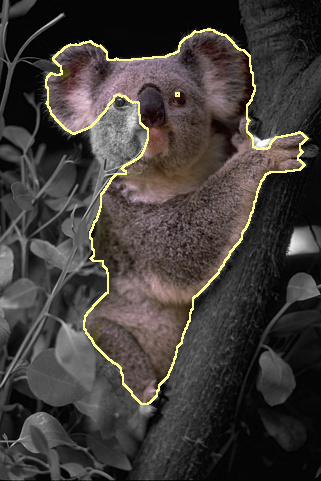
\includegraphics[scale=0.25]{figures/chapter8/segmentation/coala/k-0.0/corrected-seg.png} &  	
 	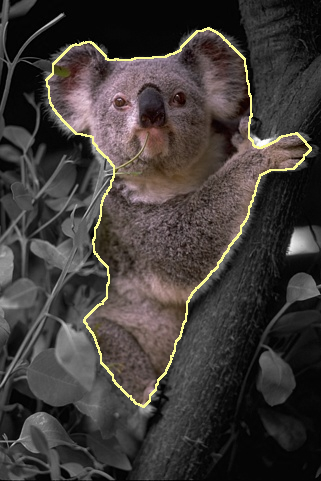
\includegraphics[scale=0.25]{figures/chapter8/segmentation/coala/k-1.0/corrected-seg.png}
\end{tabular}	
\caption{Given foreground (green) and background (gray) seeds at picture (a); GrabCut produces picture (b) which is used as input of the GraphFlow Contour Correction algorithm; in pictures (c) and (d) we display the output of Contour Correction algorithm with and without squared curvature regularization. }
\label{fig:ch8-segmentation}
\end{figure}
